\section{Discussion}
\label{sec:Discussion}
% Our claims
The asymptotic dynamics of our model are affected by the strength of intraspecific competition compared to interspecific competition. Interestingly, we find that competition closer to neutrality leads to chaotic behaviour. This suggests that in a system with predation, near-neutrality at the competition level may increase the probability of complex dynamics if the species are not equally prone to predation. Provided that the competitive exclusion principle rests on the assumption of equilibrium, near-neutrality reduces the chances of the principle to be applicable, improving the chance for a higher number of coexisting species if dynamics are chaotic \cite{Huisman1999}. Additionaly, this observation suggests that the hypothesis of non-equilibrium and Hubbell's hypothesis of neutrality are not completely independent. Our model shows another local maximum for the probability of chaos for weak competition coupling. We consider this a reasonable result, as predation is known to be the main driver of chaos in this kind of models \cite{Scheffer2004}.

%% Limitations
% Why two levels?
In the spirit of mathematical modelling, we chose the simplest realization required for the effects to be observed. We didn't use Allee effect, nor noise, and the functional form of each term has been chosen to account for satiation and saturation in the simplest possible ways. The choice of a two-level model may seem in contradiction with the pursue of simplicity, but actually it is a fundamental requirement for the effect under research to take place. In the absence of a predator level, chaos will never develop in a model with neutral competition. The reason for this is that if all interactions become equally strong, the differences among species at the same trophic level fade out. This makes labeling each species meaningless, and thus the prey-only system can be reduced just to one differential equation, that of the total prey population (see Online Appendix for details). Using the Poincaré-Bendixson theorem, it can be proven that autonomous systems with less than $3$ dimensions cannot exhibit chaos \cite{Strogatz1994}.

% Choice of interaction parameters: modularity
For simplicity, both the competition and predation parameters were drawn from probability distributions. The interactions in our system can be interpreted as a weighted network with a high connectivity. In nature, trophic networks tend to show modular structure with various clusters \cite{Thebault2010}. Our simplified model could be interpreted as representing one of the densely connected modules.

% Choice of interaction parameters: randomness
It is known that the asymptotic behaviour of this kind of systems can be very sensitive to the parameters choice. In particular, introducing correlations between parameters can greatly modify the probabilities of chaotic attractors to be reached (see for instance \cite{Huisman2001}, in response to the letter \cite{Schippers2001}). In the present paper we didn't introduce any correlation, i.e., all our random parameters were drawn independently from the others. Studying the effect of different physiological scenarios (in the sense of \cite{Huisman2001}, that is, constrains between the parameters) on the probabilities of chaos could be a continuation to this paper.

% Chaos detection
Due to the large number of simulations made, we had to rely on automatic methods for detecting chaos. Automatic detection of chaos by numerical methods has fundamental limitations, especially for high dimensional systems like ours. Most of them can be boiled down to the fact that, in general, numerical methods cannot distinguish robustly between long, complicated transients and genuine chaos. We think that our approach to chaos detection, despite being open to improvement, suffices to detect the overall patterns.

% Concluding remark
Our results suggest a fundamentally new way in which near-neutrality may promote biodiversity. In addition to weakening the forces of competitive exclusion \cite{Scheffer2018}, our analyses reveal that near neutrality may boost the chances for chaotic dynamics. As chaos in turn may facilitate super-saturated co-existence, our findings point to a potentially widespread mechanism of maintaining biodiversity.

\begin{figure}
	\begin{center}
		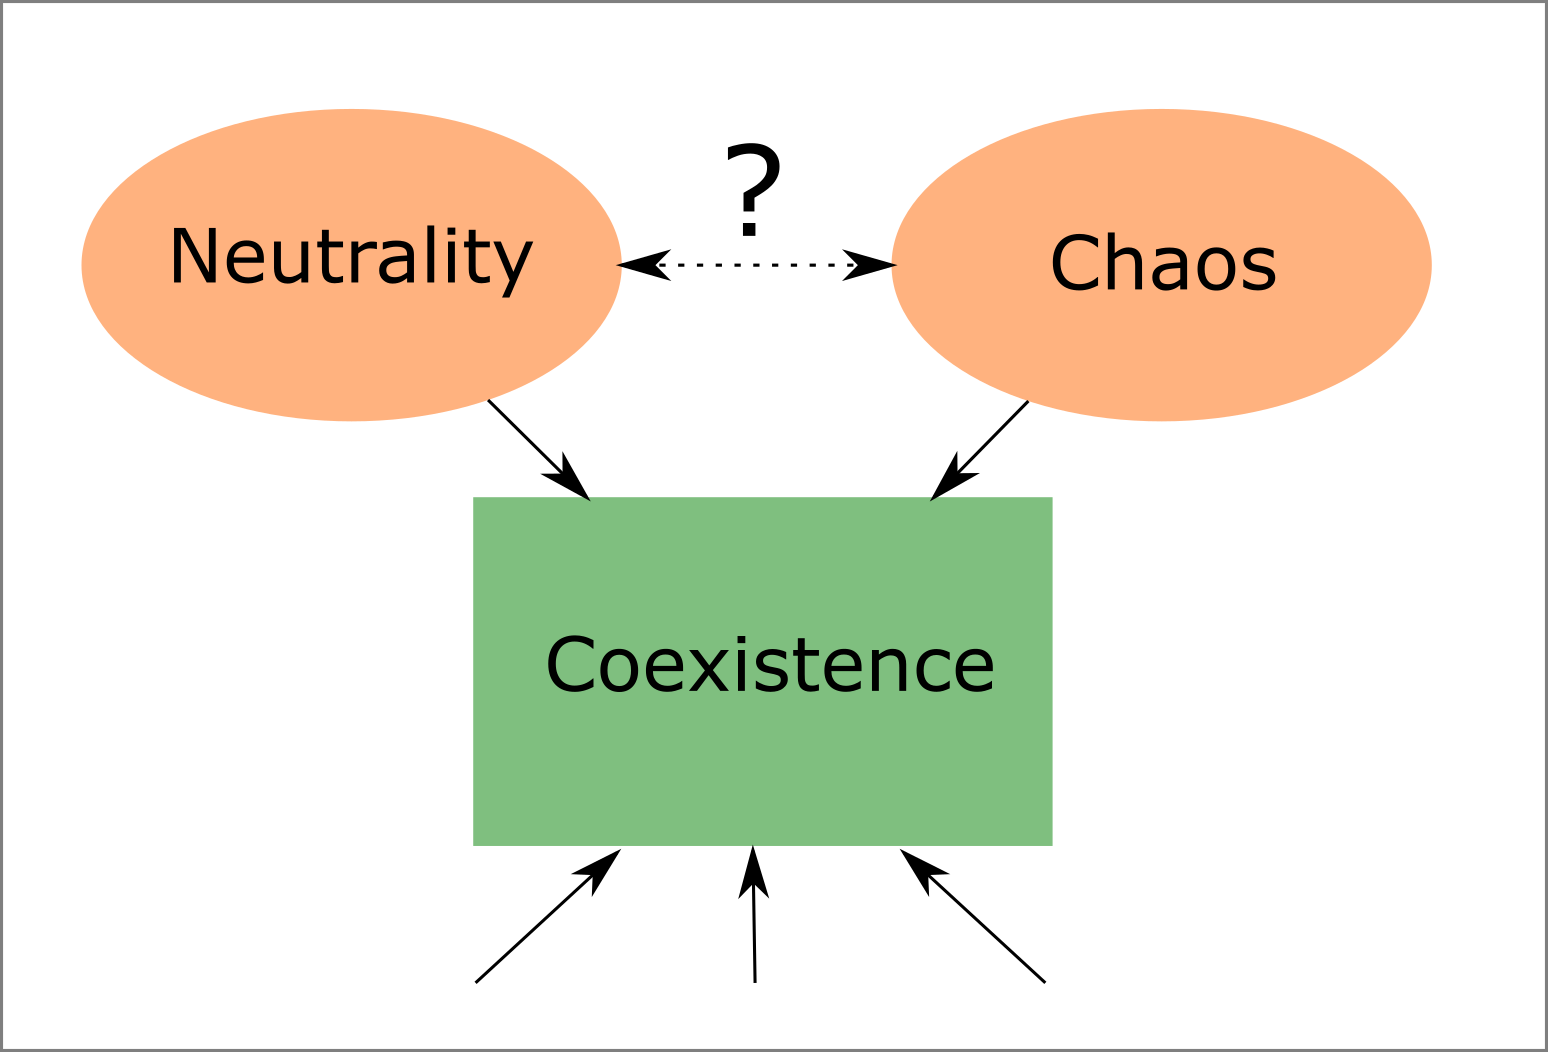
\includegraphics[width=0.5\columnwidth]{graphical_abstract.png}
	\end{center}
	\caption{In our model, neutrality and chaos are not independent explanations of coexistence.}
	\label{fig:GapInKnowledge}
\end{figure}